\chapter{Configuring Overleaf with Full LaTeX Package Support}

\small{\textit{-- Spurthi Setty}}
\label{Chapter:OverleafConfiguration}
\index{Chapter!OverleafConfiguration}

\section{Introduction}

In order to compile LaTeX documents with advanced packages such as \verb|tikz|, \verb|pgfplots|, and \verb|minted|, it is necessary to configure Overleaf's self-hosted Docker environment with the full \TeX{} Live distribution. This chapter outlines the complete setup process, including Docker configuration, LaTeX package installation, troubleshooting missing packages, and environment adjustments to ensure Overleaf compiles documents without errors.

\section{Setting Up Overleaf with Docker}

We used the official \verb|sharelatex/sharelatex| Docker image as a base and extended it with the full \TeX{} Live distribution to ensure comprehensive package support.

\subsection{Directory Structure}

All files were placed under:

\begin{minted}{bash}
/opt/overleaf/
\end{minted}

Key files include:

\begin{itemize}
  \item \texttt{Dockerfile} – to install \texttt{texlive-full}
  \item \texttt{docker-compose.yml} – to define Overleaf, MongoDB, and Redis services
\end{itemize}

\subsection{Dockerfile}

The Dockerfile extends the base image and installs \TeX{} Live:

\begin{minted}{dockerfile}
FROM sharelatex/sharelatex:latest

USER root

RUN apt-get update && \
    apt-get install -y texlive-full && \
    apt-get clean && rm -rf /var/lib/apt/lists/*

ENV TEXMFROOT=/usr/share/texlive
ENV TEXMFVAR=$TEXMFROOT/texmf-var
ENV TEXMFSYSVAR=$TEXMFROOT/texmf-var
ENV TEXMFCONFIG=$TEXMFROOT/texmf-config
ENV TEXMFSYSCONFIG=$TEXMFROOT/texmf-config
ENV TEXMFLOCAL=$TEXMFROOT/texmf-local
ENV TEXMFDIST=$TEXMFROOT/texmf-dist
ENV TEXMFHOME=/root/texmf

RUN mktexlsr
\end{minted}

\subsection{docker-compose.yml}

The Docker Compose configuration links Overleaf with MongoDB and Redis:

\begin{minted}{yaml}
services:
  sharelatex:
    image: overleaf-fulltex
    container_name: sharelatex
    restart: unless-stopped
    ports:
      - "8090:80"
    environment:
      OVERLEAF_SITE_URL: "http://<YOUR_SERVER_IP>:8090"
      OVERLEAF_MONGO_URL: "mongodb://mongo/sharelatex"
      OVERLEAF_REDIS_HOST: "redis"
    volumes:
      - overleaf_app_data:/var/lib/overleaf

  mongo:
    image: mongo:6.0
    container_name: overleaf-mongo-1
    restart: unless-stopped
    volumes:
      - overleaf_mongo_data:/data/db
    command: ["mongod", "--replSet", "rs0", "--bind_ip_all"]

  redis:
    image: redis:7
    container_name: overleaf-redis-1
    restart: unless-stopped
    command: ["redis-server", "--appendonly", "yes"]
    volumes:
      - overleaf_redis_data:/data

volumes:
  overleaf_app_data:
  overleaf_mongo_data:
  overleaf_redis_data:
\end{minted}

\subsection{Enabling MongoDB Replica Set}

Overleaf requires MongoDB to support transactions, which are only available in replica sets. After container startup, we enabled the replica set manually:

\begin{minted}{bash}
docker exec -it overleaf-mongo-1 mongosh
> rs.initiate()
\end{minted}

\subsection{Building and Starting Containers}

After creating the Dockerfile and docker-compose.yml, we built the custom image:

\begin{minted}{bash}
cd /opt/overleaf
docker build -t overleaf-fulltex .
\end{minted}

Then started all services:

\begin{minted}{bash}
docker-compose up -d
\end{minted}

\subsection{Verifying Initial Package Availability}

After building and starting the containers, we confirmed that LaTeX packages such as \verb|tikz|, \verb|pgfplots|, and \verb|psfrag| were available by executing:

\begin{minted}{bash}
docker exec -it sharelatex kpsewhich tikz.sty
docker exec -it sharelatex kpsewhich pgfplots.sty
docker exec -it sharelatex kpsewhich psfrag.sty
\end{minted}

If no path was returned, we updated the environment variables inside the container to point to the correct \TeX{} Live installation path and rebuilt the file name database with:

\begin{minted}{bash}
docker exec -it sharelatex mktexlsr
\end{minted}

\section{Troubleshooting Missing LaTeX Packages}

After successfully deploying Overleaf with the full \TeX{} Live distribution, we encountered several missing package errors when attempting to compile a Cornell University thesis template. This section documents the systematic troubleshooting process used to identify and install missing LaTeX packages.

\subsection{Initial Environment Configuration}

Our Overleaf deployment consisted of three Docker containers running on an Ubuntu virtual machine hosted on Digital Ocean:

\begin{itemize}
  \item \texttt{sharelatex} – Overleaf application server (image: \texttt{overleaf-fulltex})
  \item \texttt{overleaf-mongo-1} – MongoDB 6.0 database
  \item \texttt{overleaf-redis-1} – Redis 7 cache server
\end{itemize}

The containers were accessible via port 8090 on the host machine at \texttt{http://167.99.54.162:8090}, running \TeX{} Live 2025.

\subsection{Verifying Container Status}

Before beginning troubleshooting, we verified that all containers were running properly:

\begin{minted}{bash}
docker ps
\end{minted}

Expected output:

\begin{minted}{text}
CONTAINER ID   IMAGE              COMMAND           CREATED      STATUS      PORTS                    NAMES
7244bdc99c8a   overleaf-fulltex   "/sbin/my_init"   2 hours ago  Up 2 hours  0.0.0.0:8090->80/tcp     sharelatex
9b8786881b61   redis:7            "docker-entry..."  2 hours ago  Up 2 hours  6379/tcp                 overleaf-redis-1
3f1ee20cf169   mongo:6.0          "docker-entry..."  2 hours ago  Up 2 hours  27017/tcp                overleaf-mongo-1
\end{minted}

\subsection{Sequential Package Installation}

\subsubsection{Missing Package: \texttt{psfrag}}

The first compilation error indicated a missing \verb|psfrag.sty| file:

\begin{minted}{text}
! LaTeX Error: File `psfrag.sty' not found.

Type X to quit or <RETURN> to proceed,
or enter new name. (Default extension: sty)

Enter file name: 
! Emergency stop.
\end{minted}

We verified whether the package was already installed:

\begin{minted}{bash}
docker exec -it sharelatex tlmgr info psfrag
\end{minted}

The output confirmed the package was installed, but the \TeX{} filename database needed updating:

\begin{minted}{bash}
docker exec -it sharelatex mktexlsr
\end{minted}

We verified the package file location:

\begin{minted}{bash}
docker exec -it sharelatex find /usr/local/texlive -name "psfrag.sty"
\end{minted}

Result: \texttt{/usr/local/texlive/2025/texmf-dist/tex/latex/psfrag/psfrag.sty}

Finally, we restarted the container:

\begin{minted}{bash}
docker restart sharelatex
\end{minted}

\subsubsection{Missing Package: \texttt{fancyvrb}}

After resolving the \verb|psfrag| issue, compilation failed with:

\begin{minted}{text}
LaTeX Error: File `fancyvrb.sty' not found.
\end{minted}

We installed the missing package directly:

\begin{minted}{bash}
docker exec -it sharelatex tlmgr install fancyvrb
docker exec -it sharelatex mktexlsr
\end{minted}

\subsubsection{Missing Package: \texttt{algorithmic}}

The next compilation attempt failed at line 40:

\begin{minted}{text}
! Emergency stop.
<read *> 
         
l.40 \usepackage{algorithmic}^^M
\end{minted}

The \verb|algorithmic| package is part of the \verb|algorithms| collection:

\begin{minted}{bash}
docker exec -it sharelatex tlmgr install algorithms
docker exec -it sharelatex mktexlsr
\end{minted}

\subsubsection{Missing Package: \texttt{txfonts}}

Further compilation revealed a missing font package:

\begin{minted}{text}
LaTeX Error: File `txfonts.sty' not found.
\end{minted}

We attempted to install the font package:

\begin{minted}{bash}
docker exec -it sharelatex tlmgr install txfonts helvetic times courier
docker exec -it sharelatex updmap-sys
docker exec -it sharelatex mktexlsr
\end{minted}

However, after installation, a font error occurred:

\begin{minted}{text}
dftex error: pdflatex (file utmb8a.pfb): cannot open Type 1 font
file for reading

==> Fatal error occurred, no output PDF file produced!
\end{minted}

The \verb|txfonts| package caused persistent font mapping issues. We resolved this by commenting out the package in the document preamble:

\begin{minted}{latex}
% Line 55 in itManual.tex
%\usepackage{txfonts}
\end{minted}

For documents requiring Times-style fonts, a modern alternative can be used:

\begin{minted}{latex}
\usepackage{newtxtext,newtxmath}
\end{minted}

To use this alternative, install the package first:

\begin{minted}{bash}
docker exec -it sharelatex tlmgr install newtx
docker exec -it sharelatex mktexlsr
\end{minted}

\subsection{Installing Complete Package Collections}

Installing packages individually became inefficient as each compilation attempt revealed a new missing package. To avoid this iterative process, we installed comprehensive package collections.

We installed the \verb|collection-latexextra| collection, which includes hundreds of commonly-used LaTeX packages:

\begin{minted}{bash}
docker exec -it sharelatex tlmgr install collection-latexextra
\end{minted}

This collection includes packages such as:

\begin{itemize}
  \item \verb|fancyvrb| – Sophisticated verbatim text handling
  \item \verb|algorithmic| – Algorithm typesetting
  \item \verb|algorithm2e| – Alternative algorithm package
  \item \verb|listings| – Source code formatting
  \item \verb|tcolorbox| – Colored and framed text boxes
  \item \verb|enumitem| – Customizable list environments
  \item And many others
\end{itemize}

After installation, we updated the filename database:

\begin{minted}{bash}
docker exec -it sharelatex mktexlsr
\end{minted}

\subsection{Compiler Configuration}

Initial compilation used the \verb|latex| compiler, which generates DVI output. This caused hyperref warnings:

\begin{minted}{text}
Package hyperref Warning: You have enabled option `breaklinks'.
But driver `hdvips.def' does not support this.
\end{minted}

We changed the compiler in the Overleaf web interface:

\begin{enumerate}
  \item Navigate to \textbf{Menu} (top left corner)
  \item Under \textbf{Settings}, locate \textbf{Compiler}
  \item Change from \texttt{LaTeX} to \textbf{pdfLaTeX}
  \item Click \textbf{Recompile}
\end{enumerate}

This resolved the hyperref driver warnings and enabled direct PDF generation.

\subsection{Document-Level Fixes}

\subsubsection{Header Height Adjustment}

The \verb|fancyhdr| package warned that the header height was too small:

\begin{minted}{text}
Package fancyhdr Warning: \headheight is too small (14.45377pt): 
Make it at least 26.14003pt.
\end{minted}

We added the following line after \verb|\usepackage{fancyhdr}| in the preamble:

\begin{minted}{latex}
\usepackage{fancyhdr}
\setlength{\headheight}{27pt}
\end{minted}

\subsubsection{Hyperref Deprecated Options}

We removed deprecated options from the \verb|hyperref| package declaration. Original code:

\begin{minted}{latex}
\usepackage[pdfmark, 
breaklinks=true, 
colorlinks=true,
citecolor=blue,
linkcolor=blue,
menucolor=black,
pagecolor=black,
urlcolor=blue
]{hyperref}
\end{minted}

Updated code:

\begin{minted}{latex}
\usepackage[
breaklinks=true, 
colorlinks=true,
citecolor=blue,
linkcolor=blue,
urlcolor=blue
]{hyperref}
\end{minted}

\subsubsection{PDF Bookmark Unicode Warning}

Line breaks (\verb|\\|) in chapter or section titles cannot be included in PDF bookmarks. We used an optional argument for the PDF bookmark:

\begin{minted}{latex}
\chapter[Short Title for PDF]{Long Title \\ With Line Break}
\end{minted}

\subsection{Persistence of Installed Packages}

Docker containers are ephemeral by design. Without additional steps, all installed packages would be lost when the container is restarted. After all packages were successfully installed, we committed the container to a new Docker image:

\begin{minted}{bash}
docker commit sharelatex overleaf-fulltex-complete
\end{minted}

We then modified the \verb|docker-compose.yml| file to reference the new image:

\begin{minted}{yaml}
services:
  sharelatex:
    image: overleaf-fulltex-complete  # Changed from overleaf-fulltex
    container_name: sharelatex
    # ... rest of configuration
\end{minted}

After updating the configuration, we restarted the containers:

\begin{minted}{bash}
docker-compose down
docker-compose up -d
\end{minted}

\section{Final Working Configuration}

After completing all troubleshooting steps and package installations, the Cornell thesis template compiled successfully without errors. Figure~\ref{fig:overleaf-working} shows the final working Overleaf instance with the successfully compiled document.


\begin{figure}
    \centering
    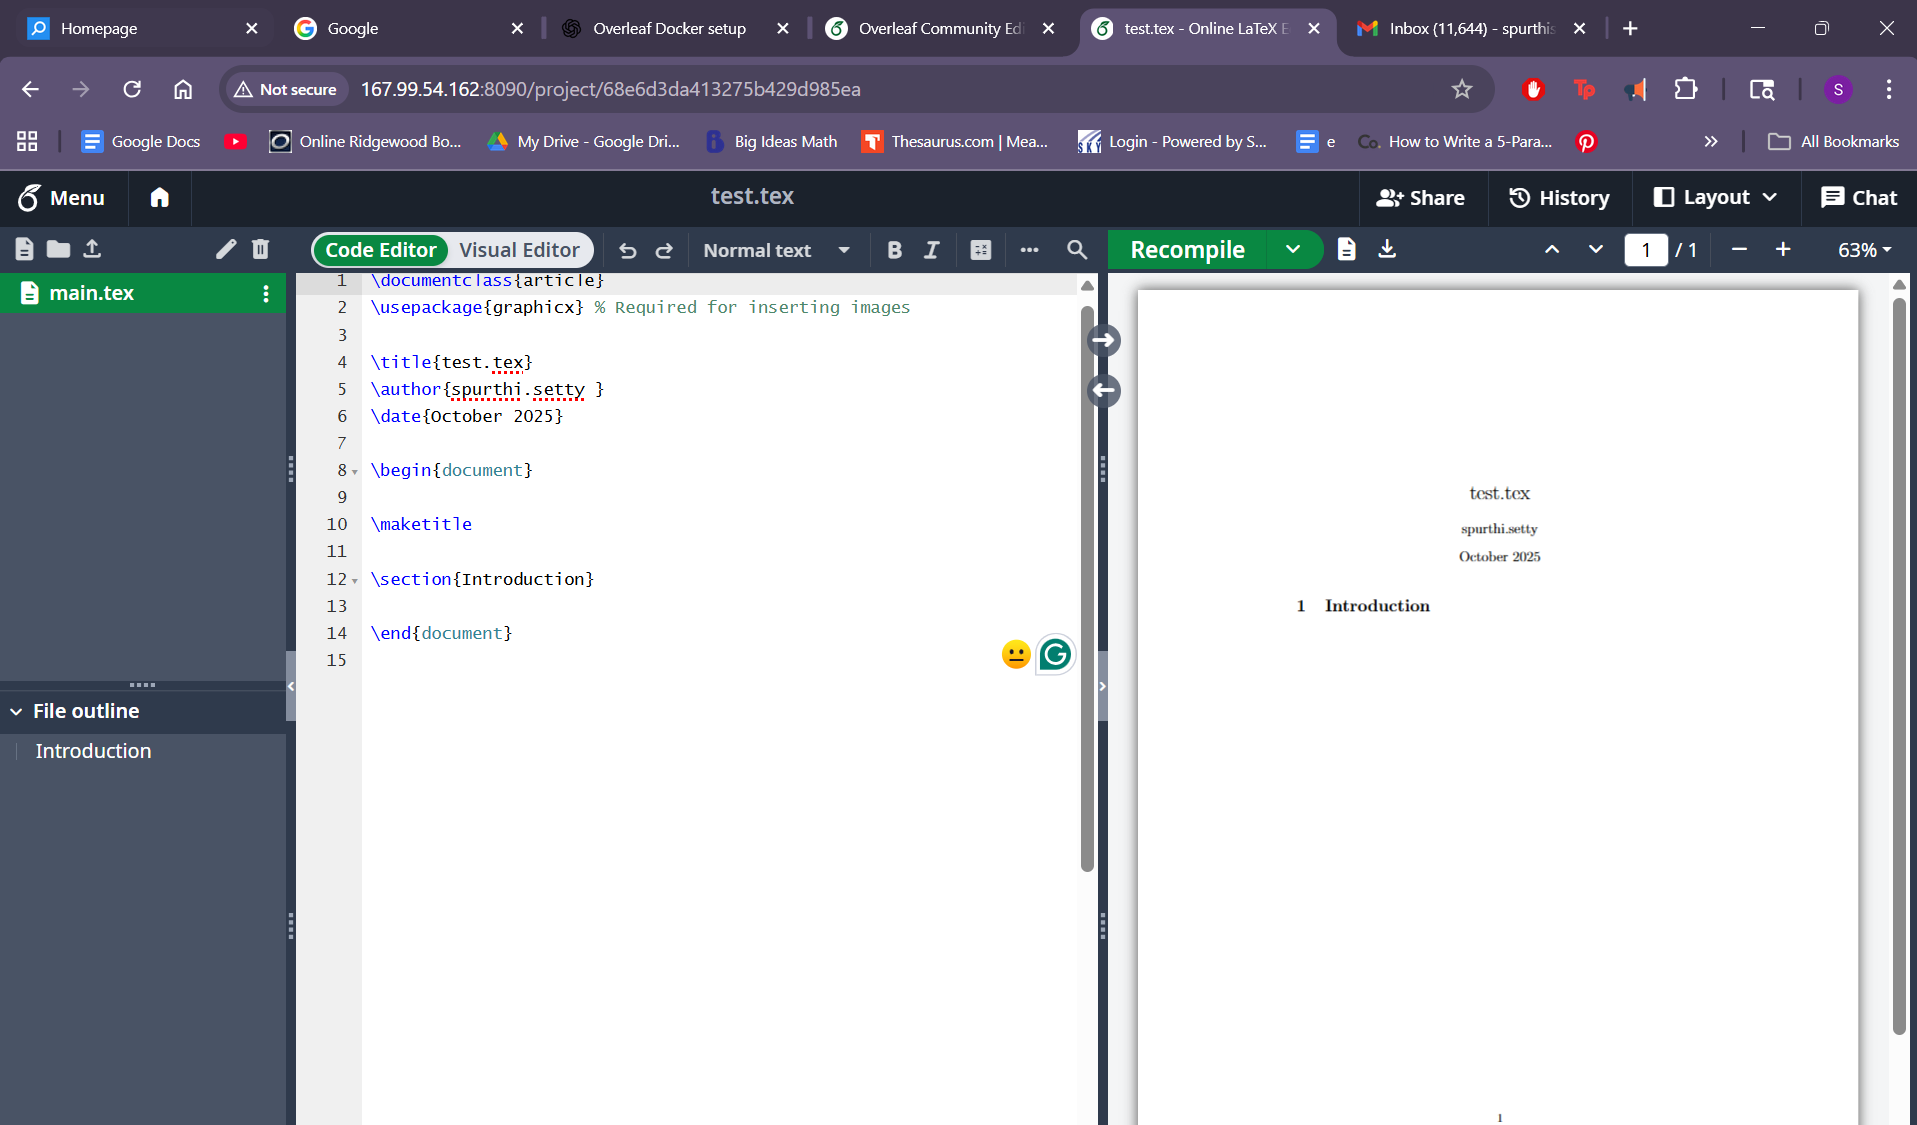
\includegraphics[width=0.9\linewidth]{png/overleaf.png}
    \caption{Successfully compiled template in Overleaf showing the PDF output, \url{URL: http://167.99.54.162:8090/project/68eed5f5ba6fdc86c648466b}}
    \label{fig:placeholder}
\end{figure}


The deployment is accessible at:

\begin{center}
\url{http://167.99.54.162:8090/project/68eed5f5ba6fdc86c648466b}
\end{center}

Key indicators of successful configuration include:

\begin{itemize}
  \item All packages load without errors
  \item PDF compiles successfully with pdfLaTeX
  \item No missing package warnings
  \item Headers and footers render correctly
  \item Hyperlinks function properly in the PDF
  \item All bibliography and index features work as expected
\end{itemize}

